% Foliensatz: "AFu-Kurs nach DJ4UF" von DK0TU, Amateurfunkgruppe der TU Berlin
% Lizenz: CC BY-NC-SA 3.0 de (http://creativecommons.org/licenses/by-nc-sa/3.0/de/)
% Autoren: Martin Deutschmann <martin.deutschmann@campus.tu-berlin.de>


\documentclass[aspectratio=169]{beamer}

\usepackage[ngerman]{babel} % deutsche Worttrennung etc.
\usepackage[utf8]{inputenc} % UTF8 Text

\usepackage[super, comma, numbers, square, sort]{natbib}

\usepackage{hyperref}       % Hyperref Package für bessere Referenzen (todo)
\hypersetup{
	colorlinks=false,       %   false: boxed links; true: colored links
    %linkcolor=white,       %   color of internal links (change box color with linkbordercolor)
    citecolor=red,          %   color of links to bibliography
    filecolor=white,        %   color of file links
    urlcolor=blue           %   color of external links
}

\usepackage{multirow}
\usepackage{wasysym}  % Math Symbols like \permil
%\usepackage{colortbl}
%\usepackage{subscript}
%\usepackage{caption}
%\usepackage{setspace}
%\usepackage{xcolor}        % benutze CodeListe

% Footnote
%\usepackage{hanging}
%
%\setbeamertemplate{footnote}{%
%  \hangpara{2em}{1}%
%  \makebox[2em][l]{\insertfootnotemark}\footnotesize\insertfootnotetext\par%
%}


%\usepackage{pgf}
%\usepackage{tikz}
%\usetikzlibrary{arrows,automata}
%\usetikzlibrary{positioning}
%
%\tikzset{
%    state/.style={
%           rectangle,
%           rounded corners,
%           draw=black, very thick,
%           minimum height=2em,
%           minimum width=2pt,
%           inner sep=2pt,
%           text centered,
%           },
%}

%\usepackage{listings}
%\lstset{basicstyle=\small, numberstyle=\tiny, extendedchars=true, numbers=left, numbersep=5pt}
%\lstset{showtabs=false, showspaces=false, showstringspaces=false}
%%\lstset{backgroundcolor=\color{white!75!lightgray}, , frame=single}
%%\lstset{backgroundcolor=\color{white}}
%%\lstset{backgroundcolor=none}
%\lstset{keywordstyle=\color{blue!50!gray},  identifierstyle=\color{black}}
%\lstset{commentstyle=\color{green!50!gray}, stringstyle=\color{red!50!gray}}
%\lstset{language=C, fontadjust=true, tabsize=2, breaklines=true}
%\lstset{backgroundcolor=\color{white!75!lightgray}, caption=\lstname, frame=single}
%\lstset{emphstyle=\color{black}\fbox}
%
%% Keine "Listing:"-Caption
%\captionsetup{labelformat=empty,labelsep=none}
%
%% für mathematische Umgebungen
%\usepackage{amsmath,amsfonts,amssymb}
%
%\lstdefinestyle{Bash}{
%language=Bash,
%frame=single,
%rulecolor=\color{black},
%backgroundcolor=\color{gray!50},
%keywordstyle=\color{black},
%identifierstyle=,
%commentstyle=\color{black},
%stringstyle=\color{magenta!65!white},
%showstringspaces=false,
%basicstyle=\footnotesize\ttfamily\color{black},
%numbers=none,
%breaklines=true,
%captionpos=b
%}

%\usepackage{listings}
%
%\lstdefinestyle{basic}{
%    captionpos=t,%
%    basicstyle=\footnotesize\ttfamily,%
%    numberstyle=\tiny,%
%    numbers=left,%
%    stepnumber=1,%
%    frame=single,%
%    showspaces=false,%
%    showstringspaces=false,%
%    showtabs=false,%
%    %
%    keywordstyle=\color{blue},%
%    identifierstyle=,%
%    commentstyle=\color{gray},%
%    stringstyle=\color{magenta}%
%}



% fließende Boxen haben keinen Abstand
%\fboxsep0mm

% inkludiere Creative Commons Helper
%%%%%%%%%%%%%%%%%%%%%%%%%%%%%%%%%%%%%%%%%%%%%%%%%%%%%%%%%%%%%%%%
%% ccBeamer 0.1, 2007-07-02                                   %%
%% Written by Sebastian Pipping <webmaster@hartwork.org>      %%
%% ---------------------------------------------------------- %%
%% Licensed under Creative Commons Attribution-ShareAlike 3.0 %%
%% http://creativecommons.org/licenses/by-sa/3.0/             %%
%%%%%%%%%%%%%%%%%%%%%%%%%%%%%%%%%%%%%%%%%%%%%%%%%%%%%%%%%%%%%%%%


%% Images
\newcommand{\CcImageBy}[1]{%
	
\includegraphics[scale=#1]{texdata/creative_commons/cc_by_30.pdf}%
}
\newcommand{\CcImageCc}[1]{%
	
\includegraphics[scale=#1]{texdata/creative_commons/cc_cc_30.pdf}%
}
\newcommand{\CcImageDevNations}[1]{%
	
\includegraphics[scale=#1]{texdata/creative_commons/cc_dev_nations_30.pdf}%
}
\newcommand{\CcImageNc}[1]{%
	
\includegraphics[scale=#1]{texdata/creative_commons/cc_nc_30.pdf}%
}
\newcommand{\CcImageNd}[1]{%
	
\includegraphics[scale=#1]{texdata/creative_commons/cc_nd_30.pdf}%
}
\newcommand{\CcImagePd}[1]{%
	
\includegraphics[scale=#1]{texdata/creative_commons/cc_pd_30.pdf}%
}
\newcommand{\CcImageSa}[1]{%
	
\includegraphics[scale=#1]{texdata/creative_commons/cc_sa_30.pdf}%
}
\newcommand{\CcImageSampling}[1]{%
	
\includegraphics[scale=#1]{texdata/creative_commons/cc_sampling_30.pdf}%
}
\newcommand{\CcImageSamplingPlus}[1]{%
	
\includegraphics[scale=#1]{texdata/creative_commons/cc_sampling_plus_30.pdf}%
}


%% Groups
\newcommand{\CcGroupBy}[2]{% zoom, gap
	\CcImageCc{#1}\hspace*{#2}\CcImageBy{#1}%
}
\newcommand{\CcGroupByNc}[2]{% zoom, gap
	\CcImageCc{#1}\hspace*{#2}\CcImageBy{#1}\hspace*{#2}\CcImageNc{#1}%
}
\newcommand{\CcGroupByNcNd}[2]{% zoom, gap
	\CcImageCc{#1}\hspace*{#2}\CcImageBy{#1}\hspace*{#2}\CcImageNc{#1}\hspace*{#2}\CcImageNd{#1}%
}
\newcommand{\CcGroupByNcSa}[2]{% zoom, gap
	\CcImageCc{#1}\hspace*{#2}\CcImageBy{#1}\hspace*{#2}\CcImageNc{#1}\hspace*{#2}\CcImageSa{#1}%
}
\newcommand{\CcGroupByNd}[2]{% zoom, gap
	\CcImageCc{#1}\hspace*{#2}\CcImageBy{#1}\hspace*{#2}\CcImageNd{#1}%
}
\newcommand{\CcGroupBySa}[2]{% zoom, gap
	\CcImageCc{#1}\hspace*{#2}\CcImageBy{#1}\hspace*{#2}\CcImageSa{#1}%
}
\newcommand{\CcGroupDevNations}[2]{% zoom, gap
	\CcImageCc{#1}\hspace*{#2}\CcImageDevNations{#1}%
}
\newcommand{\CcGroupNcSampling}[2]{% zoom, gap
	\CcImageCc{#1}\hspace*{#2}\CcImageNc{#1}\hspace*{#2}\CcImageSampling{#1}%
}
\newcommand{\CcGroupPd}[1]{% zoom
	\CcImagePd{#1}%
}
\newcommand{\CcGroupSampling}[1]{% zoom
	\CcImageSampling{#1}%
}
\newcommand{\CcGroupSamplingPlus}[1]{% zoom
	\CcImageSamplingPlus{#1}%
}


%% Text
\newcommand{\CcLongnameBy}{Attribution}
\newcommand{\CcLongnameByNc}{Attribution-NonCommercial}
\newcommand{\CcLongnameByNcNd}{Attribution-NoDerivs}
\newcommand{\CcLongnameByNcSa}{Attribution-NonCommercial-ShareAlike}
\newcommand{\CcLongnameByNd}{Attribution-NoDerivs}
\newcommand{\CcLongnameBySa}{Attribution-ShareAlike}

\newcommand{\CcNote}[1]{% longname
	This work is licensed under the \textit{Creative Commons #1 3.0 License}.%
}


% generelles Thema auswählen
\usetheme{Goettingen} %Berlin spart ohne Sidebar allerdings angenehm Platz
% AnnArbor | Antibes | Bergen | Berkeley | Berlin | Boadilla | boxes | CambridgeUS | Copenhagen | Darmstadt | default | Dresden | Frankfurt | Goettingen | Hannover | Ilmenau | JuanLesPins | Luebeck | Madrid | Malmoe | Marburg | Montpellier | PaloAlto | Pittsburgh | Rochester | Singapore | Szeged | Warsaw

% Farben wählen
\usecolortheme{beetle}
% beaver | beetle | crane | default | dolphin | dove | fly | lily | orchid | rose | seagull | seahorse | sidebartab | structure | whale | wolverine

% Setze alle Farben auf Grau und Weiß
%\definecolor{craneorange}{RGB}{64,64,64}
%\definecolor{craneblue}{RGB}{255,255,255}

% Schriftart wählen
\usefonttheme{default}
% default | professionalfonts | serif | structurebold | structureitalicserif | structuresmallcapsserif

% Innere Themen(Kopf-, Fuß-, Sidebar usw)
%\useinnertheme{default}
\useinnertheme{circles}
% default | inmargin | rectangles | rounded | circles

% Äußere Themen (Anordnung der inneren, grenzen der Folien etc.)
\useoutertheme{infolines}
% default | infolines | miniframes | shadow | sidebar | smoothbars | smoothtree | split | tree

% Deaktiviere Navigations-Symbole ({} -> leer)
\setbeamertemplate{navigation symbols}{}
%\setbeamertemplate{navigation symbols}{\large \ifnum \insertframenumber <10 0\fi\insertframenumber/\inserttotalframenumber\vspace*{0.2ex}}

% Zeige ein Hintergrundbild
\setbeamertemplate{background canvas}{
        \hspace*{-2.0cm}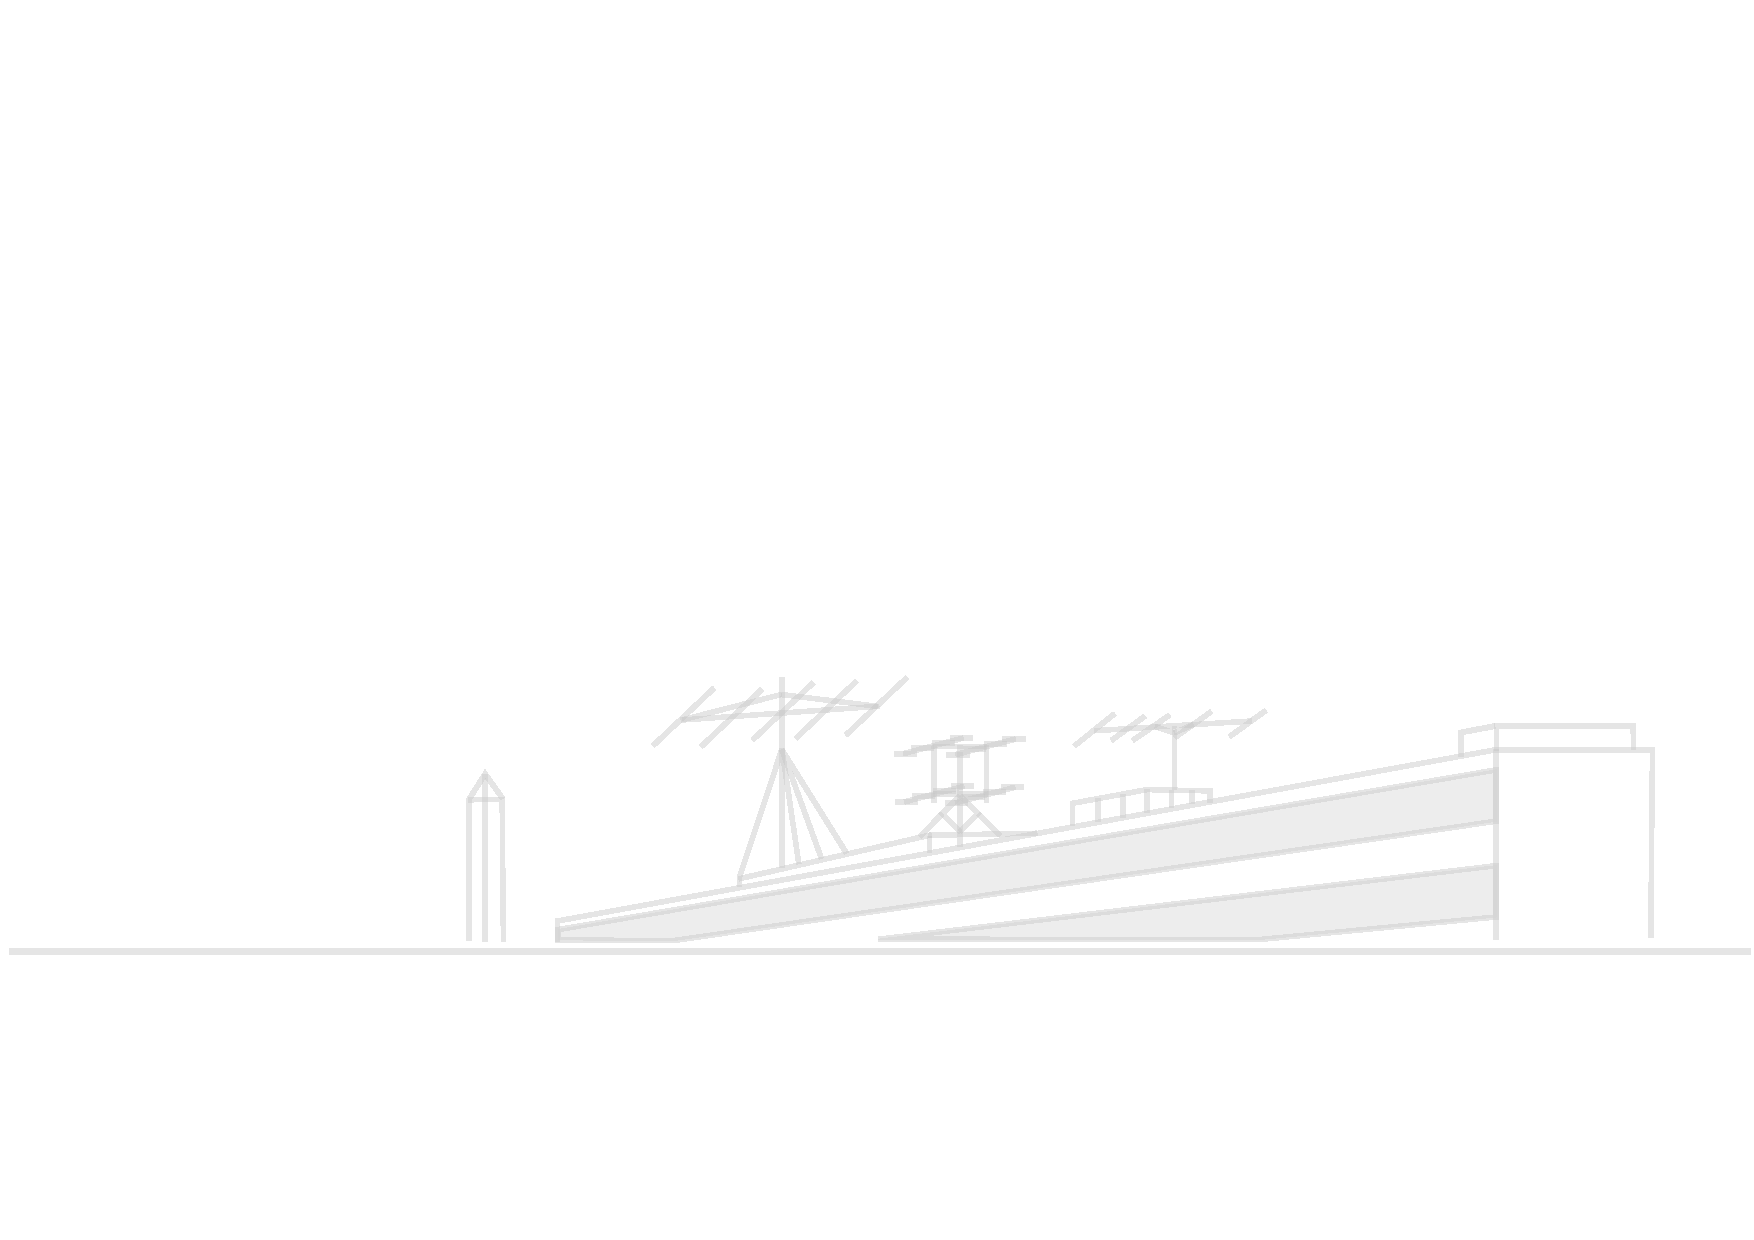
\includegraphics[width=17.8cm]{texdata/dk0tu_rooftop_background.pdf}
}

% Foliennummer einfügen
\setbeamertemplate{footline}[frame number]
%\setbeamertemplate{footline}{}

% Ändere das Zeichen vor jedem item
%\setbeamertemplate{itemize item}{\color{craneorange}$\blacktriangleright$}
%\setbeamertemplate{itemize subitem}{\color{craneorange}$\triangleright$}
%\setbeamertemplate{itemize subsubitem}{\color{craneorange}$\blacktriangleright$}

% Ändert die Blöcke 
\setbeamertemplate{blocks}[rounded][shadow=true]
% default | rounded [shadow=true|false]

%
% Eigene Kommandos
%

% Hack to get natbib and beamer working together. "The beamer user guide suggests
% that only the manual bibliography entry approach is supported"
% on some system it works out of the box, sometimes you need the hack :-(
% so check it --dl7bst
\ifdefined\newblock
    \relax
\else
    \newcommand{\newblock}{}
\fi

% \includedia command to generate png out of a dia file
% NEEDS installed dia and pdflatex option --shell-escape
\newcommand{\includedia}[1]{
    \immediate\write18{/usr/bin/dia #1.dia -e #1_diatmp.png -t png}
}

% RICHIG GROSSER FONT!
\newfont{\bigfont}{cmr10 at 144pt}
\newfont{\smallfont}{cmr10 at 8pt}

% Römische Ziffern
\makeatletter
\newcommand{\rmnum}[1]{\romannumeral #1}
\newcommand{\Rmnum}[1]{\expandafter\@slowromancap\romannumeral #1@}
\makeatother

% Schwarze Überschrift
%\setbeamercolor{frametitle}{fg=black}
%\setbeamercolor{title}{fg=black}

% Item- und Box-Farben
\definecolor{deepBlue}{HTML}{000066}
\setbeamercolor{itemize item}{fg=deepBlue}
\setbeamercolor{itemize subitem}{fg=deepBlue}
\setbeamercolor{description item}{fg=deepBlue}
\setbeamercolor{block title}{fg=deepBlue!100, bg=blue!15}
\setbeamercolor{block body}{fg=black, bg=blue!5}
\setbeamercolor{block title alerted}{fg=deepBlue, bg=red!75}
\setbeamercolor{block body alerted}{fg=black, bg=red!15}
\setbeamercolor*{block title example}{fg=blue!50, bg=blue!10}
\setbeamercolor*{block body example}{fg= blue, bg=blue!5}

%\setbeamercolor{section in head/foot}{parent=palette primary}
%\setbeamercolor{subsection in head/foot}{parent=palette secondary}
%\setbeamercolor{sidebar}{fg=darkblue,bg=yellow!90!orange}
%\setbeamercolor{title in sidebar}{fg=darkblue}
%\setbeamercolor{author in sidebar}{fg=darkblue}
%\setbeamercolor{section in sidebar}{fg=darkblue!10!black}
%\setbeamercolor{subsection in sidebar}{fg=darkblue!50!black}

% Titlepage Infos
\title{AFu-Kurs nach DJ4UF}
\author[DKØTU]{DKØTU\\ \footnotesize{Amateurfunkgruppe der TU Berlin}}
\institute[DKØTU]{\url{http://www.dk0tu.de} }

% PDF-Eigenschaften
\subject{DK0TU-Amateurfunkkurs nach DJ4UF}
\keywords{Amateurfunk Kurs HAM Radio Course CC-BY-NC-SA OpenSource TU Berlin DK0TU}

\subtitle{Technik A 16: \\
          Messtechnik \\[2em]}
\date{Stand \today}
 \begin{document}

\begin{frame}
    \titlepage
    \vfill
    \begin{center}
        \ccbyncsaeu\\
        {\tiny This work is licensed under the \em{Creative Commons Attribution-NonCommercial-ShareAlike 3.0 License}.}\\[0.5ex]
         \tiny Amateurfunkgruppe der Technische Universität Berlin (AfuTUB), DKØTU
         %\includegraphics[scale=0.5]{img/DK0TU_Logo.pdf}
    \end{center}
\end{frame}


%fixme Referenzen/Fußnoten-Systematik vereinheitlichen

\section*{Einleitung}

\begin{frame}
    \frametitle{Messgeräte}
    \begin{itemize}
		\item Was wisst ihr denn noch aus dem Kapitel E 17?
    \end{itemize}
\end{frame}

\begin{frame}
    \frametitle{Stehwellenmessgerät}
    \begin{center}
        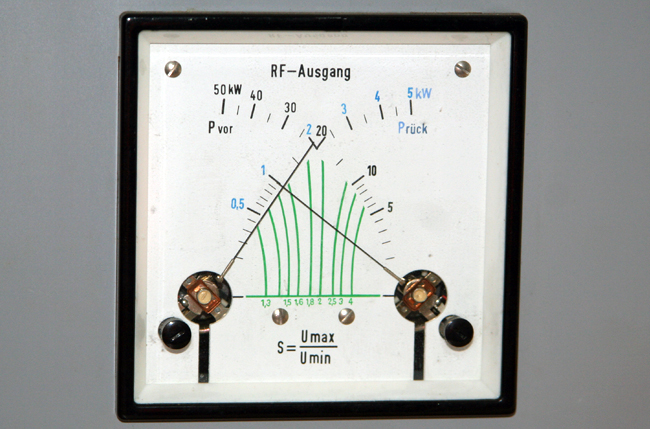
\includegraphics[width=1\textwidth]{a16/RS_SWR.jpg}\\
        Abb.1: SWR-Meter zum messen des Stehwellenverhältnisses \cite{wmen}
	\end{center}
\end{frame}

\section*{Analog}

\begin{frame}
    \frametitle{Drehspulenmessgerät (Antik)}
	\begin{minipage}{0.4\textwidth}
	    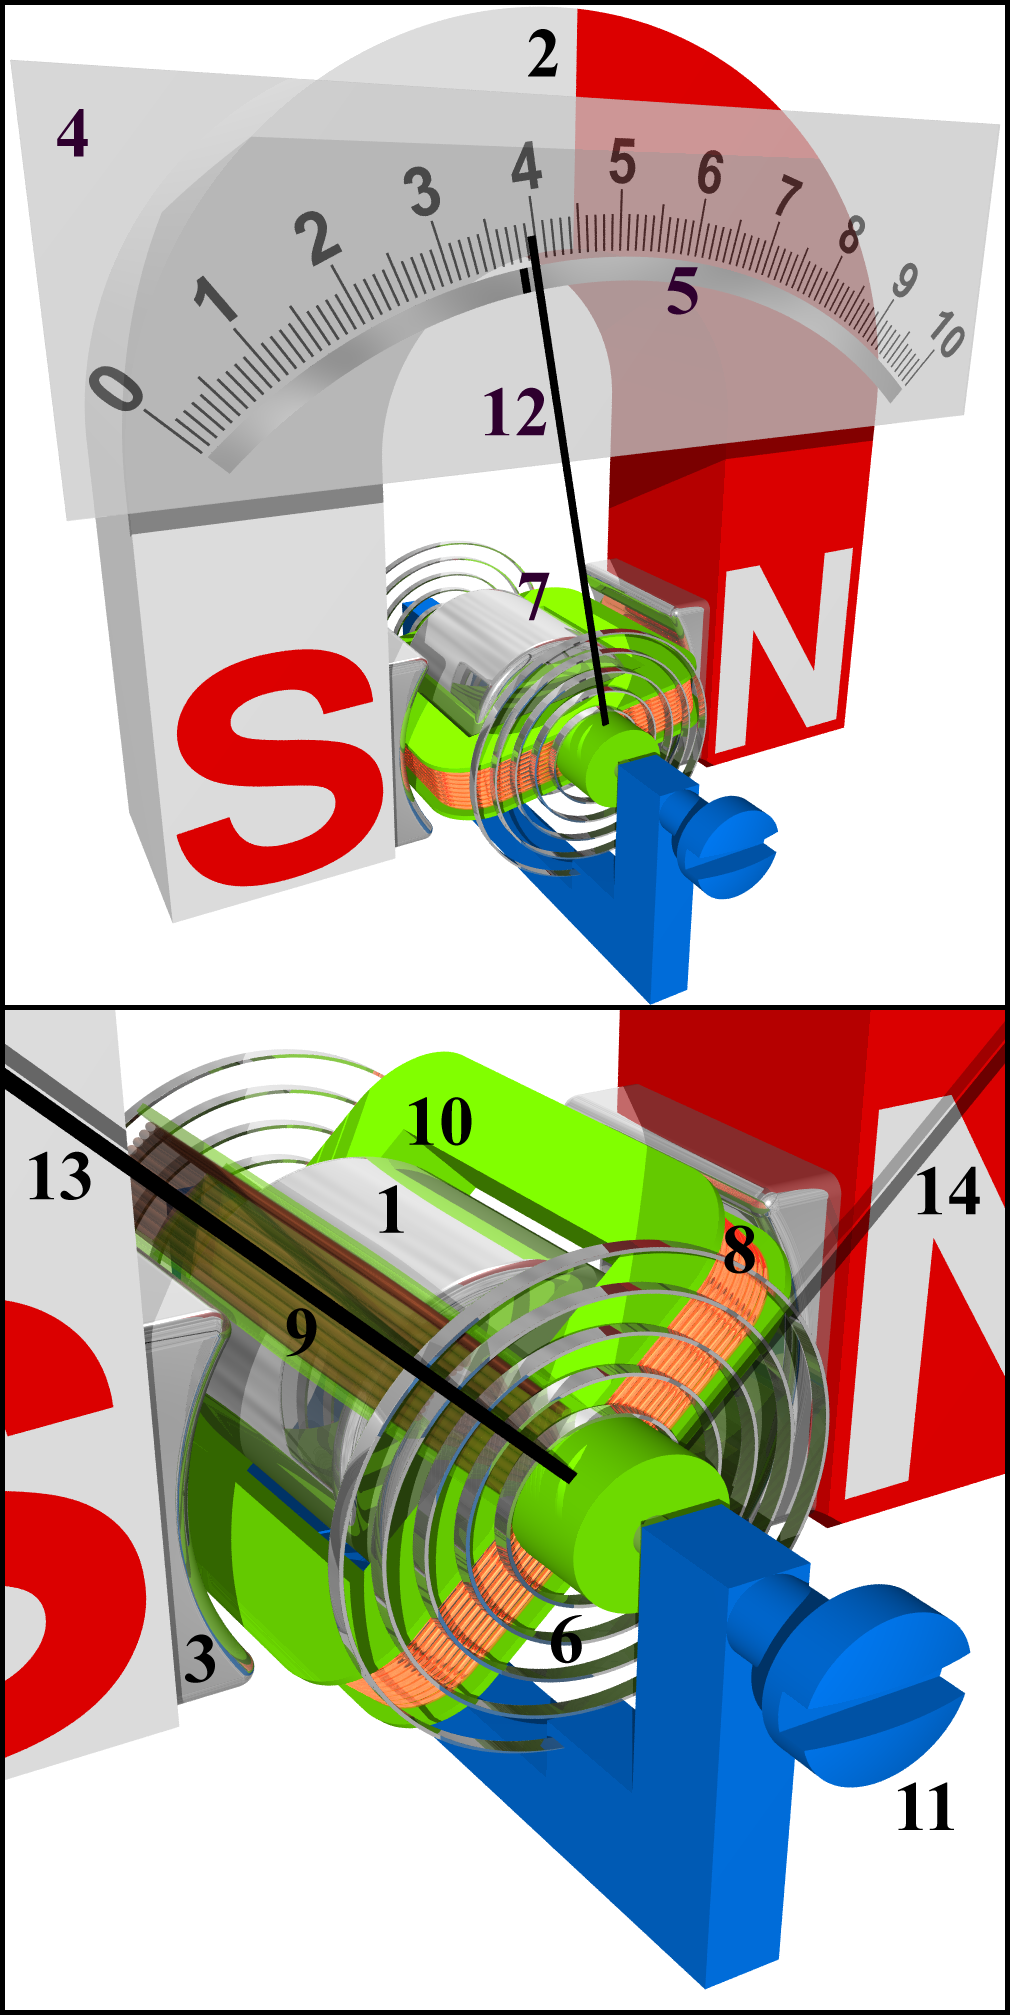
\includegraphics[width=.95\textwidth]{a16/drehspulenMess.png}
	\end{minipage}
		\hspace{0.5cm}
	\begin{minipage}{0.4\textwidth}	
	\begin{itemize} \tiny
		\item \tiny 1) Weicheisenkern der Drehspule
		\item 2) Permanentmagnet
		\item 3) Polschuh zur Bündelung des Magnetfeldes
		\item 4) Skala
		\item 5) Hilfsspiegel zur genauen Ablesung
		\item 6) Rückstellfeder
		\item 7) Drehspule
		\item 8) Drehspule in Nulllage
		\item 9) Drehspule bei Maximalausschlag
		\item 10) Joch der Spule
		\item 11) Stellschraube für Nullpunktseinstellung
		\item 12) Zeiger
		\item 13) Zeiger in Nulllage
		\item 14) Zeiger bei Maximalausschlag
	\end{itemize}
	\end{minipage}\\
	\begin{small}	
		Abb.2: Drehspulmesswerk mit Beschriftung \cite{wmen}
	\end{small}
\end{frame}

\begin{frame}
	\frametitle{Funktionsprinzip analoger Messgeräte}
	\begin{itemize}
		\item	Analoge Messgeräte funktionieren nach dem elektrodynamischen, oder dem elektrostatischen Prinzip
		\item	Dabei erzeugt die zu messende Größe ein mechanisches Drehmoment zwischen dem feststehendem Messwerk und dem beweglichen Organ
		\item	Die Empfindlichkeit wird in $k \Omega /V$ angegeben
		\item	Für Gleichstrom sollte die Empfindlichkeit bei mindestens $20 k \Omega / V$ liegen
	\end{itemize}
\end{frame}

\begin{frame}
	\frametitle{Symbole auf analogen Messgeräten}
	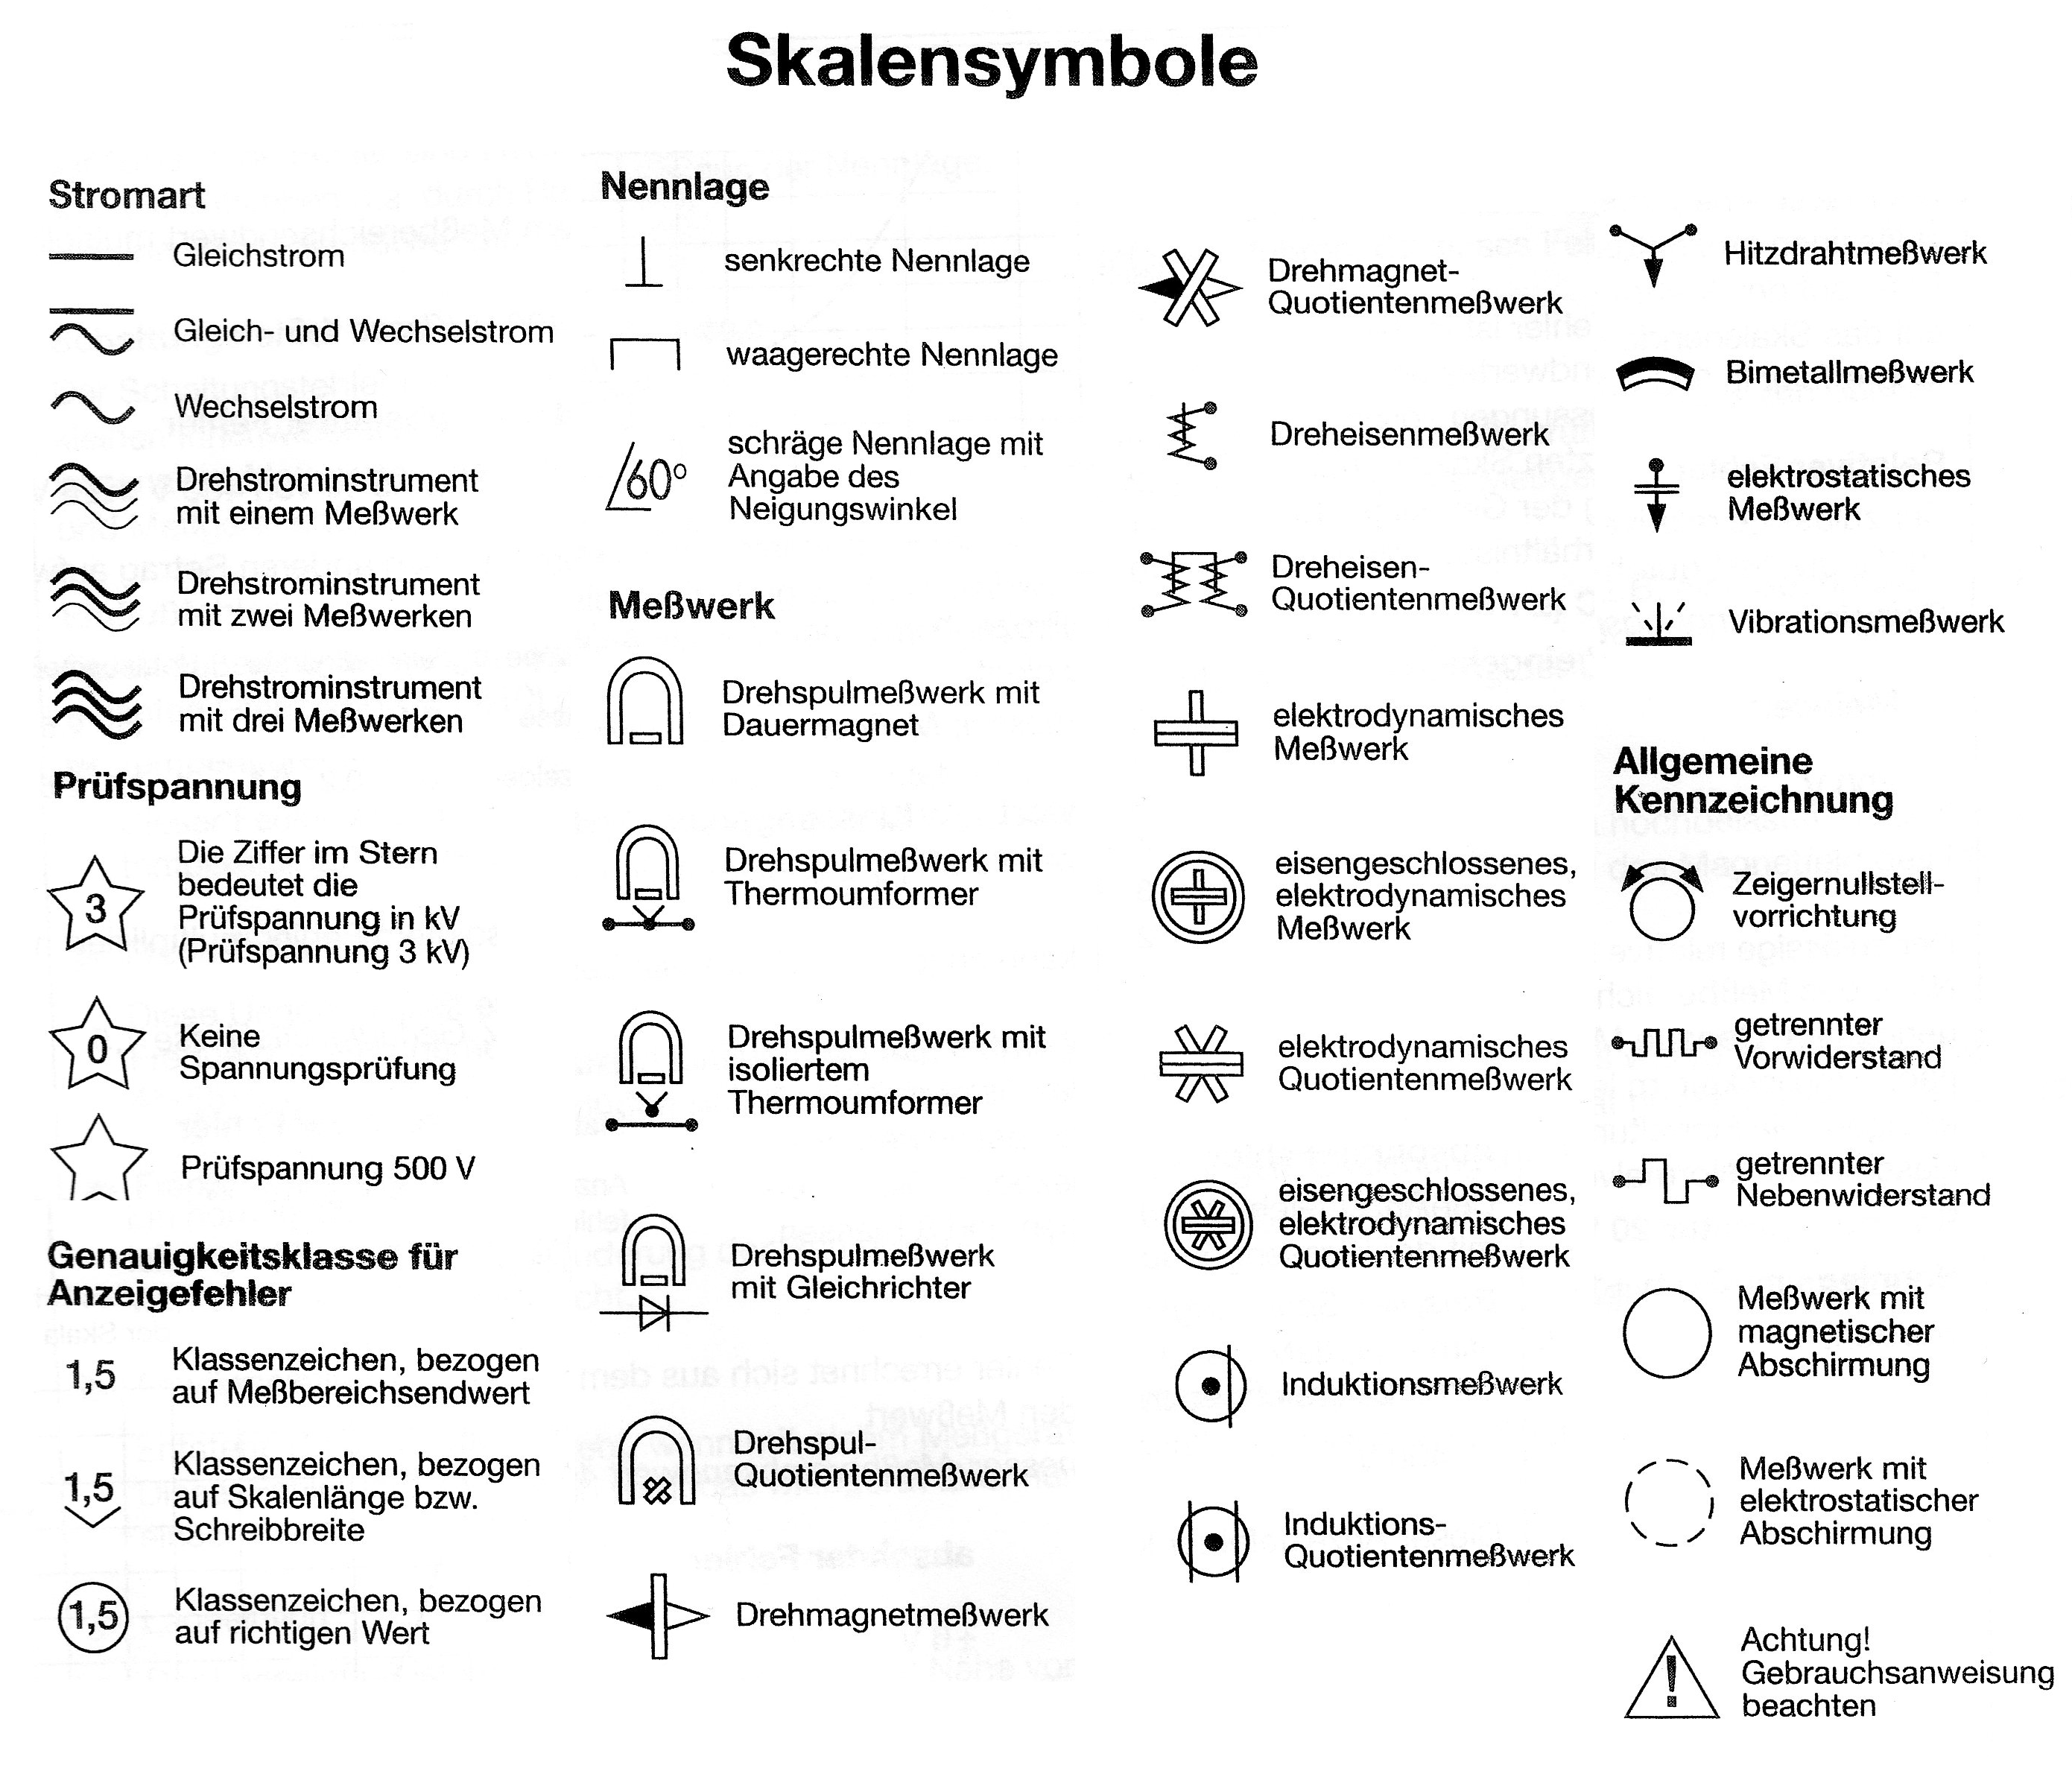
\includegraphics[scale=0.13]{a16/Symbole.png}
\end{frame}

\begin{frame}
	\frametitle{Geräteklassen}
	\begin{center}
	\begin{tabular}{|c|c|}
		\hline
		Feinmessgeräte & Betriebsmessgeräte\\ \hline
		Klasse 0.1 & Klasse 1.0 \\ \hline
		Klasse 0.2 & Klasse 1.5 \\ \hline
		Klasse 0.5 & Klasse 2.5 \\ \hline
		" " & Klasse 5.0 \\ \hline
	\end{tabular}
	\end{center}
	\begin{itemize}
		\item	Klasse gibt den prozentualen Fehler bezogen auf den Skalenendwert an
	\end{itemize}
\end{frame}

\begin{frame}
	\frametitle{Messbereichserweiterung}
	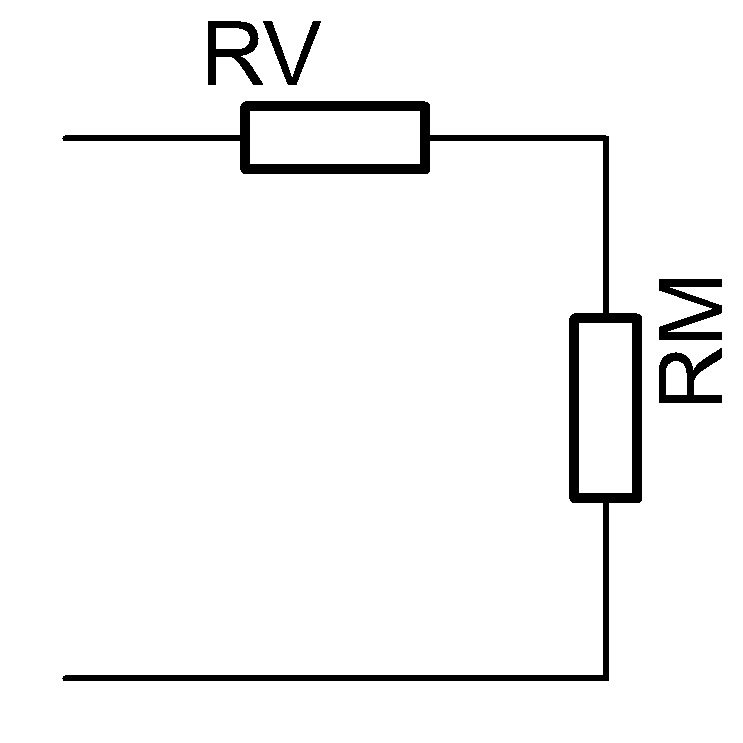
\includegraphics[scale=2]{a16/Messbereichserweiterung-Spannung.png}
	\hspace{3mm}
	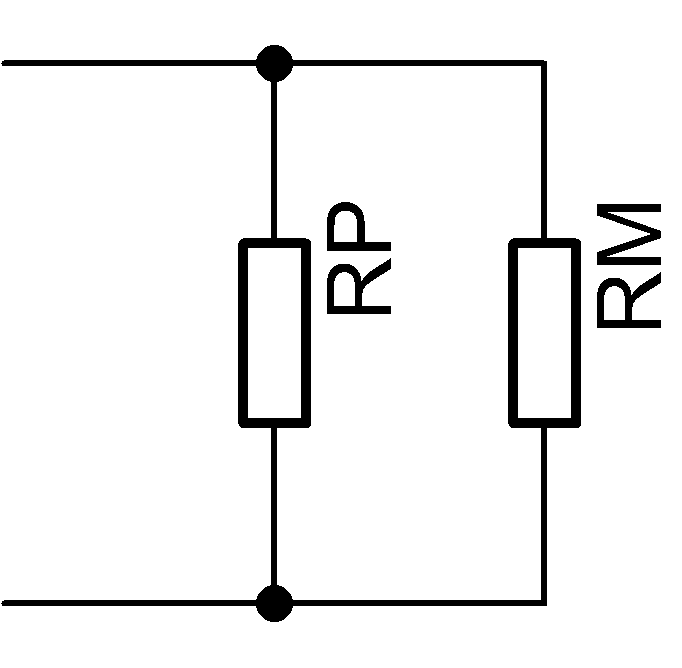
\includegraphics[scale=2]{a16/Messbereichserweiterung-Strom.png}\\
	Abb.3: Möglichkeiten zum erweitern des Messbereichs	
\end{frame}

\begin{frame}
	\frametitle{Messbereichserweiterung im Detail}
	\begin{itemize}
		\item	Sollte der Messbereich nicht ausreichen, so kann man diesen auch erweitern
		\item	Will man den Spannungsbereich erweitern, so baut man einen Vorwiderstand ein
		\item	Der Vorwiderstand und das Messgerät bilden einen Spannungsteiler
		\item	Je nach Verhältnis aus $\frac{R_M}{R_{gesamt}}$ kann man dann höhere Spannungen messen
		\item	Um den Strombereich zu erweitern, schaltet man einen Widerstand parallel zum Messgerät
		\item	Dieser sorgt dafür, das weniger Strom durch das Messgerät fließt 
	\end{itemize}
\end{frame}

\begin{frame}
	\frametitle{Messgleichrichter}
	\begin{center}
	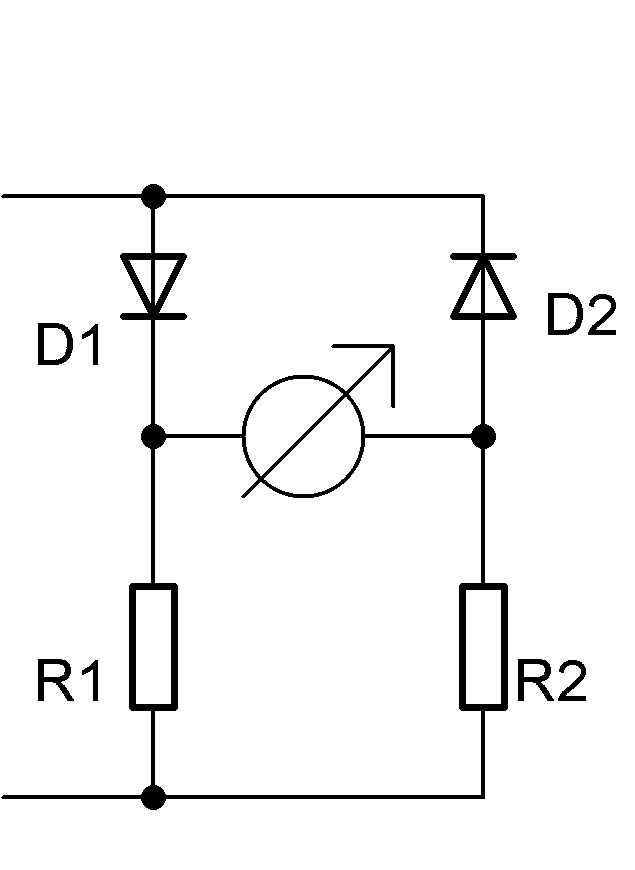
\includegraphics[scale=1.2]{a16/Messgleichrichter1.png}
	\hspace{3mm}
	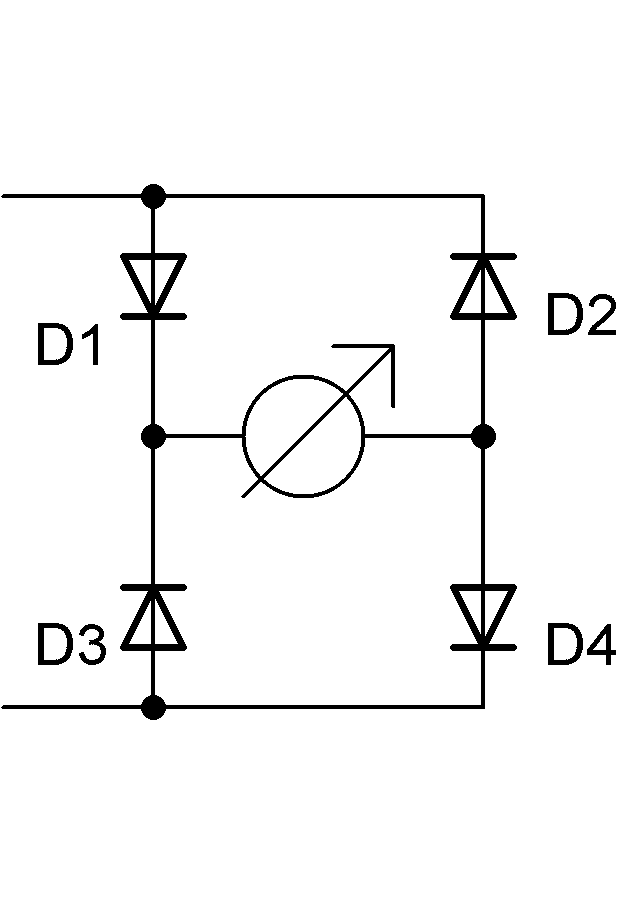
\includegraphics[scale=1.3]{a16/Messgleichrichter2.png}\\
	Abb.4: Mögliche Schaltungen für Messgleichrichter	
	\end{center}
\end{frame}

\begin{frame}
\frametitle{Messgleichrichter}
	\begin{itemize}
		\item	Drehspulmesswerke eignen sich nur zum messen von Gleichstrom
		\item	Um auch Wechselspannungen messen zu können, nutzt man Messgleichrichter
		\item	Diese funktionieren aber nur für sinusförmige Signale
		\item	Für andere Signalformen gibt es das Dreheisenmesswerk
		\item	Diese brauchen keinen Gleichrichter benötigen aber recht viel Leistung und sind nicht als Feinmessgeräte tauglich
		\item	Will man im GHz-Bereich messen benötigt man einen speziellen Thermoumformer
	\end{itemize}		
\end{frame}

\section*{Digital}

\begin{frame}
    \frametitle{Digitales Multimeter}
    \begin{minipage}{0.5\textwidth}
    \begin{center}
        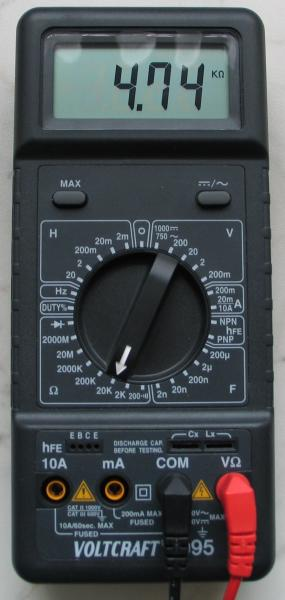
\includegraphics[width=.35\textwidth]{a16/digitalmultimeter.jpg}\\
        Abb.5: Digitales Multimeter von Voltcraft \cite{wmde}
	\end{center}
	\end{minipage}
	\begin{minipage}{0.4\textwidth}
		\begin{itemize}
			\item	Verringern Chance auf Ablesefehler
			\item	Brauchen Strom zum messen
			\item	Auflösung ist die kleinste Einteilung der Anzeige
		\end{itemize}			
	\end{minipage}
	\vspace{3mm}
	\begin{itemize}
		\item	Neben der Auflösung ist auch die Genauigkeitsklasse zu beachten
		\item	Können unter anderem Strom, Spannung, Induktivitäten, Kapazitäten, Verstärkung von Bipolartransistoren und Frequenzen messen
	\end{itemize}
\end{frame}

\begin{frame}
    \frametitle{Was wo anschließen?}
	\begin{minipage}{0.4\textwidth}
        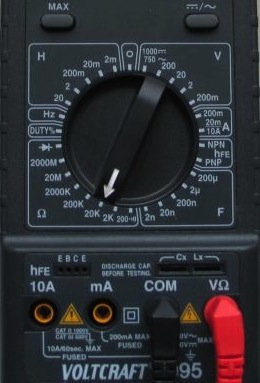
\includegraphics[width=1\textwidth]{a16/digitalmultimeterMess.jpg}
	\end{minipage}
	\begin{minipage}{0.4\textwidth}	
	\begin{itemize}
		\item Was kann alles gemessen werden?
		\item Wo anschließen zum Strom messen?
		\item Wo anschließen zum Spannung messen?
		\item Welcher Messbereich?
	\end{itemize}
	\end{minipage}
	\vspace{3mm}
	Abb.6: Wählrad und Anschlüsse eines Multimeters \cite{wmde}
\end{frame}

\begin{frame}
    \frametitle{Messfehler}
    \begin{center}
    		\begin{itemize}
				\item Nullpunktsabweichung
				\item Empfindlichkeitsabweichung
				\item Linearitätsabweichung
    		\end{itemize}
        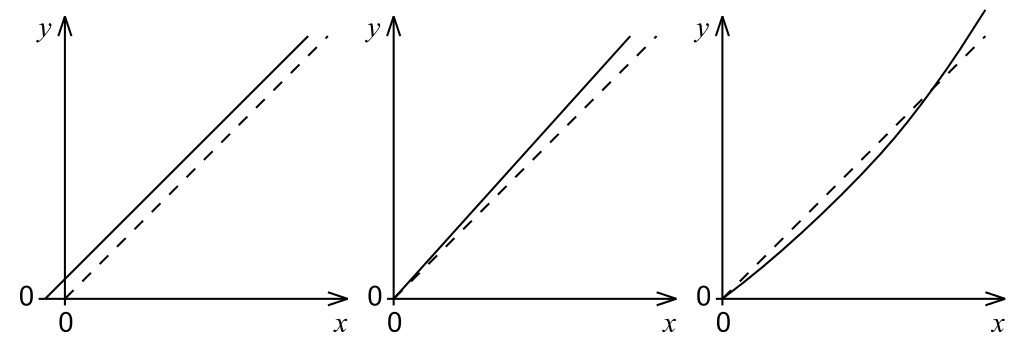
\includegraphics[width=1\textwidth]{a16/werMisstMisst.png}\\
       	Abb.7: Mögliche Abweichungen durch Messfehler \cite{wmde}
	\end{center}
\end{frame}

\section*{Oszilloscope}

\begin{frame}
    \frametitle{Oszilloscope}
    \begin{center}
        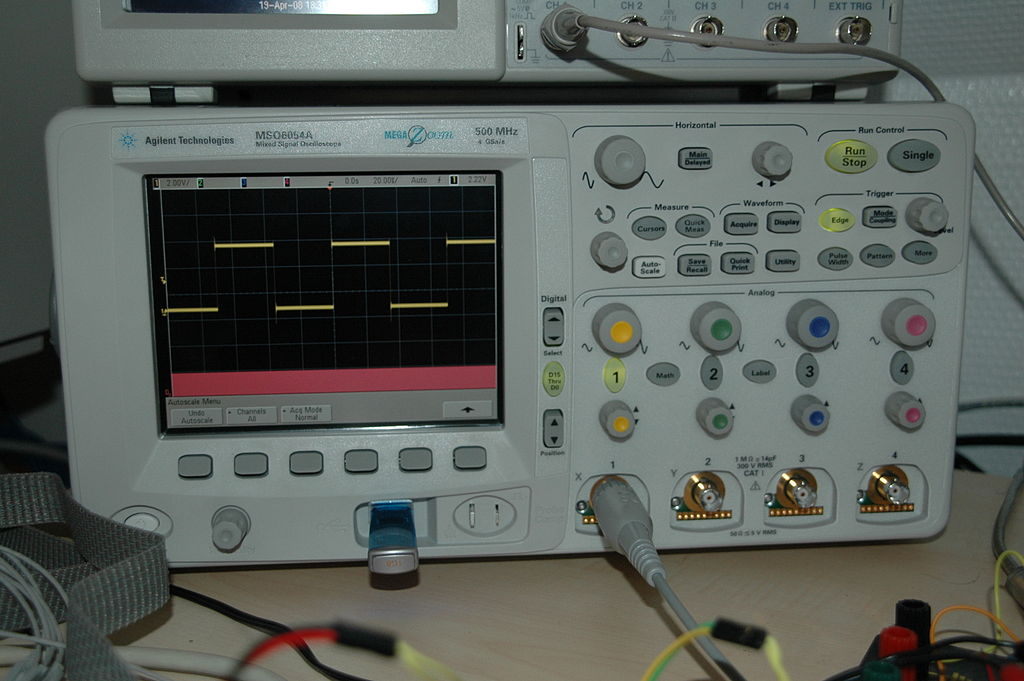
\includegraphics[width=1\textwidth]{a16/osziModern.jpg}\\
        Abb.8: Modernes Speicheroszilloskop \cite{wmde}
	\end{center}
\end{frame}

\begin{frame}
	\begin{itemize}
		\item	Können zeitliche Verläufe von Spannungen darstellen
		\item	Anzeige mit Elektronenstrahlröhre(veraltet) oder LCD(moderner)
		\item	Kann stehende Bilder von Wellen darstellen, indem die Welle immer an einem bestimmten Amplitudenwert getriggert(gestartet) wird
		\item	Benötigt dafür eine Triggereinrichtung
	\end{itemize}
\end{frame}

\begin{frame}
    \frametitle{Oszilloscope - Ablesen}
    \begin{center}
        $100mV / Div$ und $0.1ms / Div$
        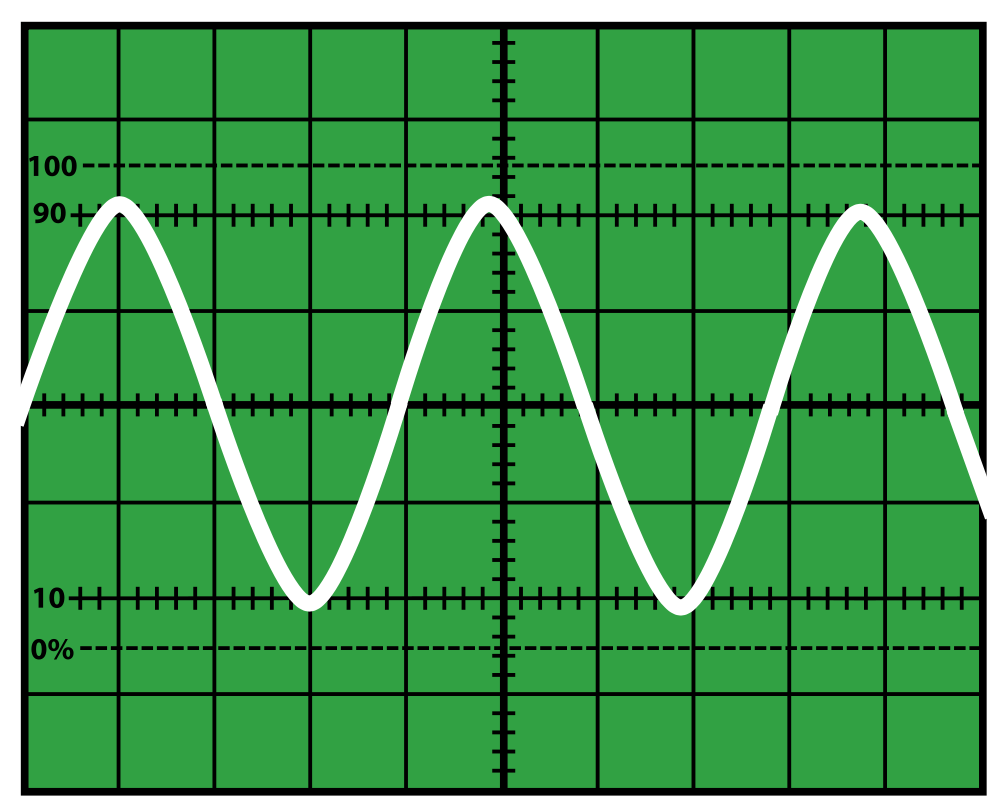
\includegraphics[width=.8\textwidth]{a16/OsziTon.png}\\
       	Abb.9: Signal auf einem Oszilloskop \cite{wmde}
	\end{center}
\end{frame}

\begin{frame}
	\frametitle{Verschiedene Signalformen}
	\begin{center}
        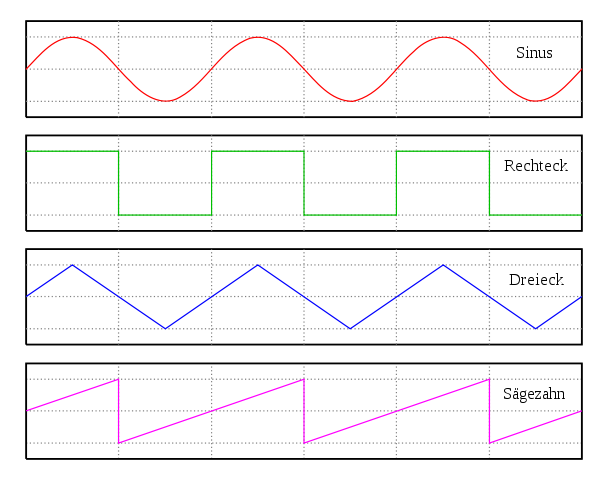
\includegraphics[width=0.95\textwidth]{a16/Signalformen.png}\\
		\begin{small}
			Abb.10: Verschiedene elementare Signalformen \cite{wmen}
		\end{small}		       
	\end{center}
\end{frame}

\begin{frame}
    \frametitle{Spannungen}
    \begin{center}
    \begin{itemize}
			\item PEP - Peak to Peak
			\item RMS - Effektivwert
			\item $u_{Spitze} = \sqrt{2} \cdot U_{eff}$ \\
			\item Aufgabe: Berechnet Spitzen-Spitzen Spannung vom Netzstrom 
    \end{itemize}
	\end{center}
\end{frame}

\section*{Absorptionsfrequenzmesser}
\begin{frame}
    \frametitle{Absorptionsfrequenzmesser}
    \begin{center}
        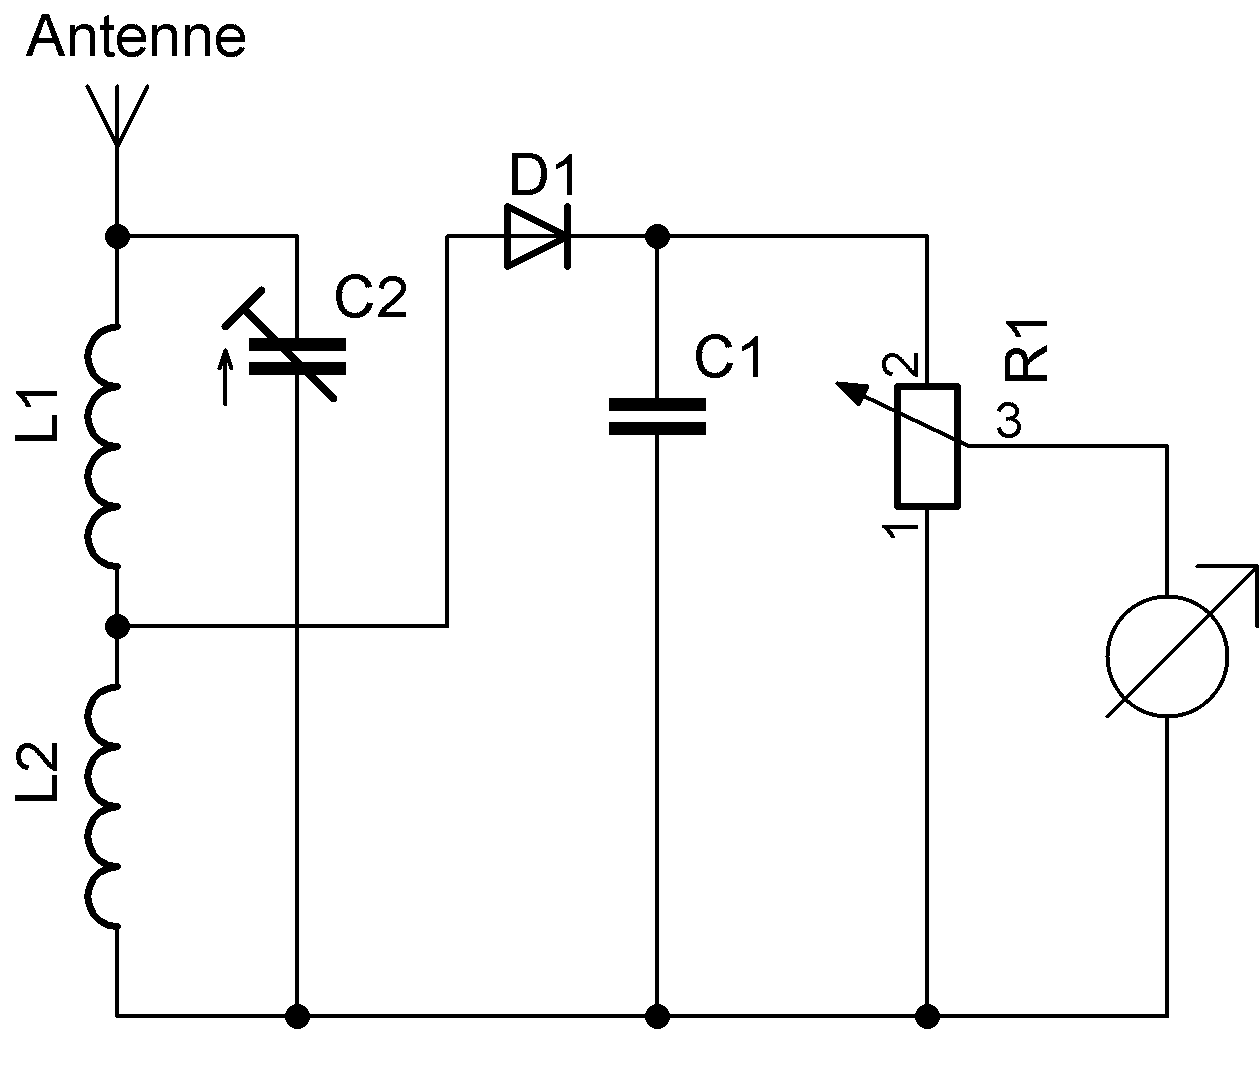
\includegraphics[width=0.5\textwidth]{a16/Absorptionsfrequenzmesser.png}\\
        Abb.11: Schaltung eines Absorptionsfrequenzmessers
	\end{center}
	\begin{itemize}
		\item	Besteht aus einem passiven Schwingkreis hoher Güte, einem AM-Demotulator und einer Antenne
		\item	Damit lassen sich passiv Senderfrequenzen und Oberwellen feststellen
		\item	Anzeigegenauigkeit liegt bei etwa 5\%
	\end{itemize}
\end{frame}

\section*{Feldstärkeanzeiger}
\begin{frame}
    \frametitle{Feldstärkeanzeiger}
    \begin{center}
        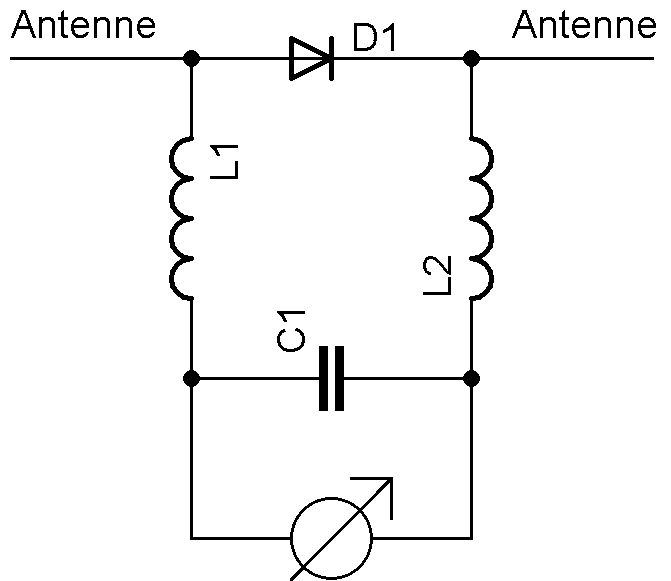
\includegraphics[width=0.6\textwidth]{a16/Feldstaerkeanzeiger.png}\\
        Abb.12: Schaltung eines Feldstärkeanzeigers
	\end{center}
	\begin{itemize}
		\item	Wird zum Prüfen(!!! nicht zum messen!!!) der Feldstärke genutzt
		\item	Besteht aus einer HF-Diode, HF-Drosseln und einem Kondensator
	\end{itemize}
\end{frame}

\section*{Dipmeter}

\begin{frame}
    \frametitle{Dipmeter}
    \begin{center}
        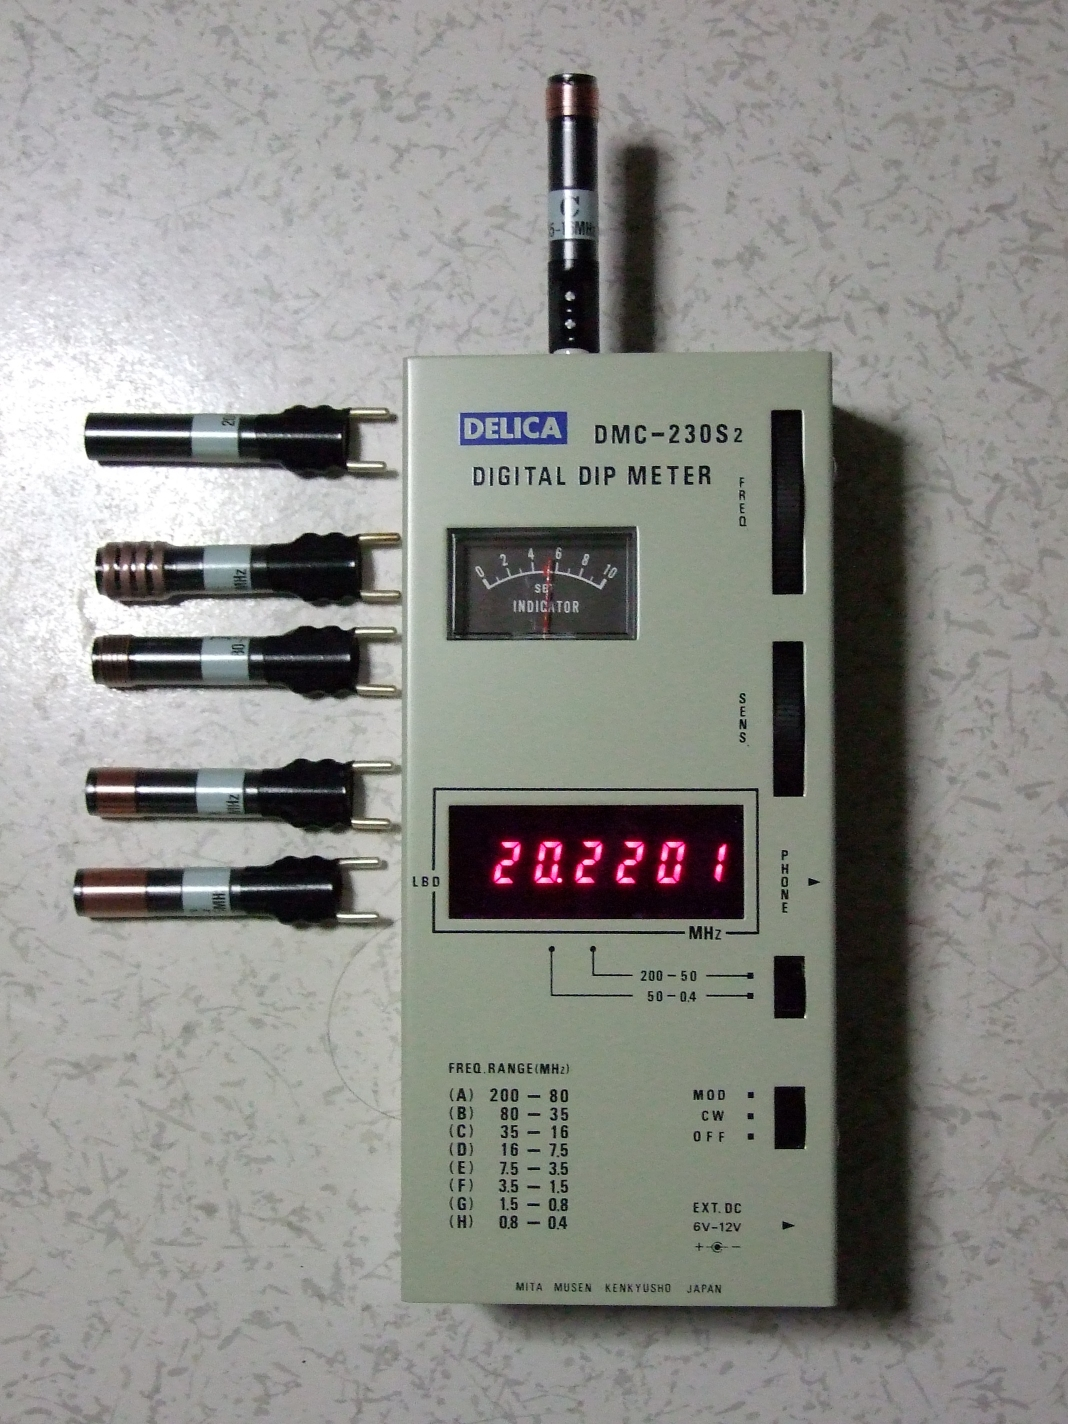
\includegraphics[width=0.55\textwidth]{a16/Dipmeter.jpg}\\
        Abb.13: Dipmeter mit beiliegenden Mess-Spulen \cite{wmen}
	\end{center}
\end{frame}

\begin{frame}
	\begin{itemize}
		\item	Ein Dipmeter ist prinzipiell ein Oszillator mit nach außen geführter Schwinkreisspule
		\item	Der Schwingkreis wird durch das Messobjekt beeinflusst
		\item	Der Rückgang der Schwingungsamplitude wird mit einer Anzeige sichtbar gemacht
		\item	Anzeigegenauigkeit liegt bei etwa 3\%
		\item	Kann indirekt eine Induktivität messen
		\item	Dafür schaltet man einen Kondensator parallel zur Induktivität, ermitteln die Resonanzfrequenz und rechnet um
		\item	Zum messen wird eine relativ lose Kopplung zwischen Dipmeter und Messobjekt benötigt
		\item	Da sonst das Messobjekt verstimmt wird und das Messergebnis dadurch verfälscht
	\end{itemize}
\end{frame}

\section*{Frequenzzähler}
\begin{frame}
    \frametitle{Frequenzzähler}
    \begin{center}
        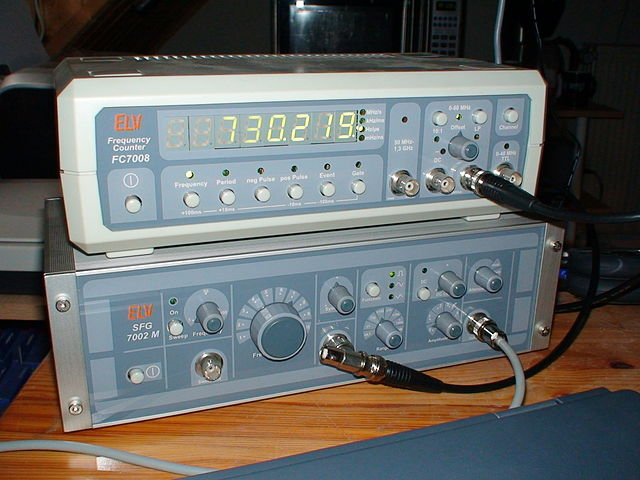
\includegraphics[width=0.6\textwidth]{a16/Frequenzzaehler.jpg}\\
        Abb.14: Frequenzzähler von ELV \cite{wmen}
	\end{center}
\end{frame}

\begin{frame}
	\begin{itemize}
		\item	Zählt während einer eingestellten Torzeit die ankommenden Impulse
		\item	Um die Genauigkeit zu erhöhen müssen mehr Impulse gezählt werden, weshalb eine längere Torzeit eingestellt werden muss
		\item	Kann keine Oberwellen messen, wenn dir Grundfrequenz noch vorhanden ist
		\item	Sehr genaue Messungen erhält man mit einer hohen Auflösung und einer temperaturstabilen Quarzzeitbasis 
		\item	Will man höhere Frequenzen messen, kann man einen Vorteiler nutzen
		\item	Meist wird dafür ein Vorteiler mit Faktor 10 benutzt
	\end{itemize}
\end{frame}

\section*{Spektrumanalysator}
\begin{frame}
    \frametitle{Spektrumanalysator}
    \begin{center}
        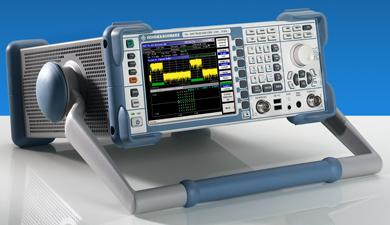
\includegraphics[width=0.6\textwidth]{a16/Spektrumanalysator.jpg}\\
        Abb.15: Beispiel eines Spektrumanalysators \cite{wp}
	\end{center}
\end{frame}

\begin{frame}
	\begin{itemize}
		\item	Kann die Amplitude eines Signals in Abhängigkeit der Frequenz darstellen
		\item	Besitzt dafür einen "Wobbeloszillator" der schnelle seine Frequenz ändern kann
		\item	Die Wobbelbandbreite kann zum messen von Oberwellen sehr breit eingestellt werden
		\item	Um Senderbandbreite zu ermitteln kann die Sie sehr schmal eingestellt werden
	\end{itemize}
\end{frame}

\begin{frame}
    \frametitle{Spektrumanalysator}
    \begin{center}
        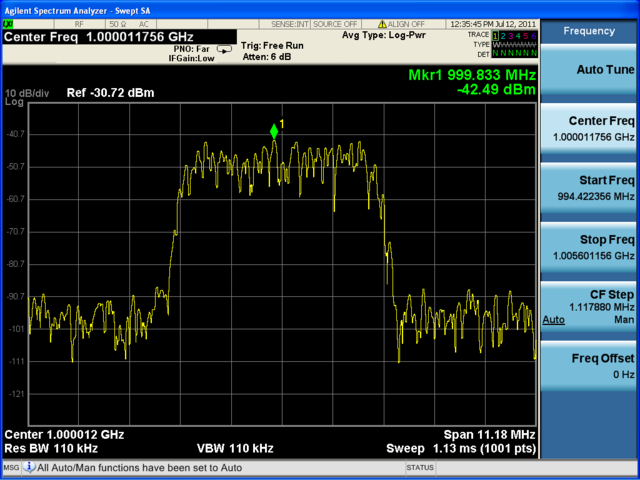
\includegraphics[width=0.6\textwidth]{a16/Spektrumanalysator-Display.png}\\
        Abb.16: Display eines Spektrumanalysators zeigt Frequenzgang \cite{wp}
	\end{center}
\end{frame}

\section*{Referenzen}

	\begin{small}
    \begin{thebibliography}{}
    \bibitem{a02}  Moltrecht A 17: \\
                    \url{http://www.darc.de/referate/ajw/ausbildung/darc-online-lehrgang/technik-klasse-a/technik-a16/}
                    
    \bibitem{wp}    Wikipedia DE: \\
    	\url{http://commons.wikimedia.org/wiki/File:FSL.jpg}\\
    	\url{http://de.wikipedia.org/wiki/Datei:SpectrumAnalyzerDisplay.png}
                    
    \bibitem{wmde}	Wikimedia DE:\\
   		\url{https://commons.wikimedia.org/wiki/File:Oszi_Ton.svg}\\
   		\url{https://commons.wikimedia.org/wiki/File:Modernes_Speicheroszilloskop.jpg}\\
   		\url{https://commons.wikimedia.org/wiki/File:AMT_Fehler.svg}\\
   		\url{http://commons.wikimedia.org/wiki/File:Digitalmultimeter.jpg}\\
   		
   	\bibitem{wmen}	Wikimedia EN:\\
   		\url{https://commons.wikimedia.org/wiki/File:Dipmeter_and_its_probe_coils.jpg}\\
   		\url{https://commons.wikimedia.org/wiki/File:RS_SWR.jpg}\\
   		\url{https://commons.wikimedia.org/wiki/File:Moving_coil_instrument_principle.png}\\
   		\url{http://commons.wikimedia.org/wiki/File:Waveforms_de.svg}
   		\url{http://commons.wikimedia.org/wiki/File:Frequency_counter.JPG}\\
   		  		
	\end{thebibliography}
	\end{small}

% Hier könnte noch eine Kontaktfolie stehen

\end{document}

